\chapter{Sentiment analysis}
\label{sentiment_analysis}
Oggigiorno siamo affetti da e produciamo un tale sovraccarico di dati che le aziende si stanno ridefinendo per raccogliere queste informazioni, come per esempio i feedback dei clienti, e strutturare il processo decisionale. L'ottenimento di questi dati è impensabile se fatto manualmente.
\par 
In particolare, per le opinioni su prodotti e servizi viene in aiuto la sentiment analysis, una discplina che può fornire risposte riguardo le questioni più importanti dal punto di vista dei clienti.
\par
Il processo di sentiment analysis permette, attraverso l'elaborazione del linguaggio naturale, di estrarre e analizzare in modo automatizzato opinioni soggettive espresse dall'utente, determinarne la polarità (positiva, neutrale, negativa) e, successivamente, riassumerle in maniera da poter essere di valore per l'azienda.
\par 
In questo modo, le decisioni possono essere prese sulla base di una quantità di dati significativa, piuttosto che da una semplice intuizione che non sempre si rivela corretta. Il rischio infatti a cui si va incontro maggiormente è quello di interpretare i messaggi avendo già un pregiudizio sull’argomento in questione, influenzando il modo in cui il testo da analizzare può essere interpretato.
\par
La sentiment analysis è importante perché le aziende vogliono che il loro marchio sia recepito positivamente (con un occhio alle aziende concorrenti). A tal proposito, ci si può concentrare su commenti positivi o negativi oltre che sul feedback del cliente, per valutare sia i punti di forza che i punti su cui migliorare.


\section{Preprocessing}
\label{preprocessing}
Prima di partire con lo svolgimento del task di sentiment analysis, è necessaria una fase di preprocessing.
\par
Innanzitutto, sono stati rimossi dal dataset i campi ritenuti superflui per l'analisi.
\par
Successivamente, è stato manipolato il campo \texttt{reviewText}. La manipolazione è avvenuta sequenzialmente e con step standard per analisi di questo tipo:

\begin{itemize}
    \item \textbf{Normalization} - conversione delle recensioni in caratteri minuscoli. Se presenti, modificate alcune espressioni contratte tipiche della lingua inglese (per esempio: \textit{hadn't} trasformata in \textit{had not}).
    \item \textbf{Tokenization} - suddivisione in token per ogni recensione
    \item \textbf{Removal} - rimozione di token altamente ricorrenti nella lingua considerata (stopwords). Inoltre, sono stati eliminati token composti da 1 o 2 caratteri o token estremamente rari (frequenza nel dataset = 1)
    \item \textbf{Lemmatization} - conversione del token nel proprio lemma linguistico
    
\end{itemize}{}

Questa manipolazione ha portato alla creazione del campo \texttt{preprocessedReview}.
Di seguito vengono mostrate la recensione originale e la recensione dopo l'intera fase di preprocessing.
\par
\begin{itemize}
  \item[\textbf{Prima}] \texttt{Overall a great product with a fair price. I have had absolutely no problems with the product except for the volume level, which is *NOT* below standard, it is just simply what is to be expected from a headset. Very comfortable, and I personally prefer the boom mic to be longer (unlike the newer models of this headset which have shortened mics). Recommended.}
  \item[\textbf{Dopo}] \texttt{overall great product fair price absolutely problem product volume level standard simply expect headset comfortable personally prefer boom mic longer new model shorten mic recommend}
\end{itemize}

\section{Creazione di Bag of Words}
\label{bow}
Il campo \texttt{preprocessedReview} non è direttamente trattabile dagli algoritmi di machine learning e quindi è necessario ottenere una rappresentazione comprensibile. 
Innanzitutto, abbiamo rimosso dall'analisi del campo \texttt{preprocessedReview} le recensioni:
\begin{itemize}
    \item prolisse - rientrano in questa categoria le osservazioni con più di 300 parole
    \item irrilevanti - rientrano in questa categoria le osservazioni con meno di 5 parole
\end{itemize}{}

Dopodiché, le recensioni restanti sono state utilizzate per costruire una Bag of Words composta da 10000 feature. Oltre ai token vengono considerati anche i bigrammi, poiché un loro utilizzo può aumentare l'accuratezza del modello rispetto al solo utilizzo di token singoli.
\section{Esplorazione}
A partire dalla nuova rappresentazione matriciale è stato creato un DataFrame fittizio composto dalle 10000 feature individuate nel Capitolo \ref{bow} e, per ognuna di esse, viene segnata la frequenza con cui appaiono rispettivamente nelle recensioni positive e nelle recensioni negative, oltre che la frequenza totale data dalla loro somma.
\par
Le recensioni neutrali non sono state considerate in quanto aggiungerebbero un livello ulteriore di complessità nell'apprendimento dei modelli.

\subsection{Wordcloud}
Una Wordcloud è una rappresentazione grafica delle parole usate di frequente in un corpus di documenti e fornisce un'idea generale di che tipologia di parole possiamo trovarvi. La grandezza di ogni parola nell'immagine è un'indicazione della frequenza di occorrenza della parola nell'intero corpus. Per questo motivo, sono molto utili quando si vuole eseguire un'analisi del testo.

\begin{figure}[H]
  \centering
  \includesvg[width=0.9\linewidth]{figures/2_wordcloud_positive}
  \caption{Wordcloud of positive reviews}
  \label{pos_wordcloud}
\end{figure}

\begin{figure}[H]
  \centering
  \includesvg[width=0.9\linewidth]{figures/2_wordcloud_negative}
  \caption{Wordcloud of negative reviews}
  \label{neg_wordcloud}
\end{figure}

\subsection{Frequenza dei token}

Un'ulteriore analisi che si può fare riguarda la distribuzione dei token all'interno del dataset. Nella Figura \ref{50_pos} e nella Figura \ref{50_neg} vengono mostrati gli istogrammi (ordinati dal token più frequente al token meno frequente) rispettivamente per le recensioni positive e le recensioni negative.
\begin{figure}[H]
  \centering
  \includesvg[width=0.8\linewidth]{figures/2_token_frequency_positive}
  \caption{Top 50 tokens in positive reviews}
  \label{50_pos}
\end{figure}

\begin{figure}[H]
  \centering
  \includesvg[width=0.8\linewidth]{figures/2_token_frequency_negative}
  \caption{Top 50 tokens in negative reviews}
  \label{50_neg}
\end{figure}

Un modello comunemente utilizzato è la legge di Zipf, ovvero una legge empirica formulata nel 1959 in cui vi si afferma che, dato un corpus di documenti, la frequenza di ogni parola è inversamente proporzionale al suo rango nella tabella delle frequenze. Pertanto, la parola più frequente ricorre approssimativamente il doppio rispetto alla seconda parola più frequente, il triplo rispetto alla terza parola più frequente e così via.

\begin{figure}[H]
  \centering
  \includesvg[width=0.8\linewidth]{figures/2_plot_frequency}
  \caption{Distribution of words in review for each opinion}
  \label{distribution_words_opinion}
\end{figure}

La legge di Zipf viene osservata più facilmente tracciando i dati su scala logaritmica in entrambi gli assi come mostrato in Figura \ref{zipf_law}.

\begin{figure}[H]
  \centering
  \captionsetup{margin=1cm}
  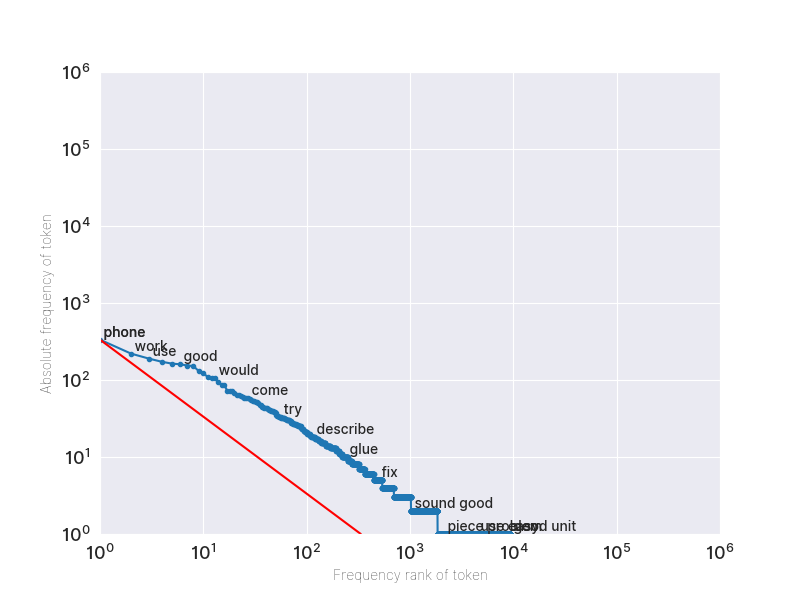
\includegraphics[width=0.8\linewidth]{figures/2_zipf_law.png}
  \caption{Distribution of words in verified reviews}
  \label{zipf_law}
\end{figure}


\section{Machine learning}
La tecnica con cui abbiamo affrontato la fase di sentiment analysis è il machine learning. Grazie ad essa il modello viene addestrato per riconoscere il sentimento in base alle parole usando un training set etichettato. Questo approccio dipende in gran parte dal tipo di algoritmo e dalla qualità dei dati utilizzati per l'addestramento.

\par
Grazie all'attenta fase di preprocessing, è stato possibile addestrare due modelli diversi con gli stessi dati e valutarne i risultati, confrontandoli.
\par
Per prima cosa abbiamo dovuto risolvere il problema dello sbilanciamento tra classi: le recensioni positive sono in numero molto maggiore rispetto a quelle negative e qualsiasi modello addestrato rischierebbe di ottimizzarsi più sulla classe maggiore.
La soluzione più adeguata in questo caso è l'utilizzo di una tecnica di undersampling in modo da ridurre gli elementi della classe maggioritaria senza introdurre bias e rendendo equiparabili le cardinalità delle classi.
\par
Il problema di machine learning è di natura binaria in quanto la variabile target ha solo due possibili valori: \textit{positive} e \textit{negative}.
Data questa semplicità ci sono numerosi modelli che possono essere addestrati. Sono stati scelti Multinomial Naive Bayes e Logistic Regression per il loro ottimo compromesso tra performance e tempo di addestramento. Abbiamo provato ad implementare anche una Support Vector Machine ma le risorse hardware richieste per l'addestramento non erano disponibili.
\par
Per entrambi i modelli è stata eseguita la tecnica di Cross Validation (CV) su 5 folds, dividendo quindi il training set in 5 sottoinsiemi e usandone uno come test set, per 5 volte.

to do:split da aggiungere
Per entrambi i modelli è stato tenuto da parte un validation set per la verifica finale e l'analisi delle varie metriche.

\subsection{Analisi dei risultati}

Al di sopra della CV è stata eseguita anche una Grid Search nel tentativo di trovare i migliori iperparametri per i due modelli.
In Naive Bayes è stato trovato il migliore valore per alpha (0.1), mentre nella Logistic Regression il migliore valore dell'iperparametro C è stato 1.
\par
Analizzando le matrici di confusione dei due modelli in Figura \ref{cm_nb} e in Figura \ref{cm_lr} notiamo che il modello di Logistic Regression individua in totale meno falsi positivi e falsi negativi rispetto a Naive Bayes; ciò è confermato dal valore di \textit{Accuracy} leggermente più alto.

\begin{figure}[H]
  \centering
  \includesvg[width=0.9\linewidth]{figures/2_confusion_matrix_nb.svg}
  \caption{Confusion Matrix per Naive Bayes}
  \label{cm_nb}
\end{figure}

\begin{figure}[H]
  \centering
  \includesvg[width=0.9\linewidth]{figures/2_confusion_matrix_lr.svg}
  \caption{Confusion Matrix per Logistic Regression}
  \label{cm_lr}
\end{figure}

\par
Sia i valori di \textit{Precision} che quelli di \textit{Recall} di Logistic Regression sono più alti indicando che per entrambe le classi tale modello trova un miglior numero di True e un minor numero di False.

\begin{table}[H]
\centering
  \begin{tabular}{l l} 
  Accuracy complessiva & 0.84\\
  Precision per la classe \textit{positive} & 0.84\\
  Precision per la classe \textit{negative} & 0.85\\
  Recall per la classe \textit{positive} & 0.85\\
  Recall per la classe \textit{negative} & 0.84\\
    \end{tabular}
    \caption{Metriche risultate dell'esecuzione della cross validation su Naive Bayes}
\end{table}

\begin{table}[H]
\centering
  \begin{tabular}{l l} 
  Accuracy complessiva & 0.87\\
  Precision per la classe \textit{positive} & 0.87\\
  Precision per la classe \textit{negative} & 0.86\\
  Recall per la classe \textit{positive} & 0.86\\
  Recall per la classe \textit{negative} & 0.88\\
    \end{tabular}
    \caption{Metriche risultate dell'esecuzione della cross validation su Logistic Regression}
\end{table}


\par
Le due ROC in Figura \ref{roc_nb} e in Figura \ref{roc_lr} mostrano l'andamento del rapporto tra True Positive Rate e False Positive Rate al variare del valore di cut-off di ogni modello: anche in questo grafico possiamo vedere una performance migliore da parte della Logistic Regression poichè la sua curva si avvicina di più a quella "ideale" e la sua inclinazione è più verticale.

\begin{figure}[H]
  \centering
  \includesvg[width=0.9\linewidth]{figures/2_roc_nb.svg}
  \caption{ROC per Naive Bayes}
  \label{roc_nb}
\end{figure}

\begin{figure}[H]
  \centering
  \includesvg[width=0.9\linewidth]{figures/2_roc_lr.svg}
  \caption{ROC per Logistic Regression}
  \label{roc_lr}
\end{figure}

